\documentclass[11pt,aspectratio=169]{beamer}

% =====================================================
% THEME AND PACKAGES
% =====================================================
\usetheme{Madrid}
\usecolortheme{default}

\usepackage[utf8]{inputenc}
\usepackage[T1]{fontenc}
\usepackage[french]{babel}
\usepackage{amsmath, amssymb}
\usepackage{booktabs}
\usepackage{array}
\usepackage{graphicx}
\usepackage{xcolor}
\usepackage{tikz}
\usepackage{tcolorbox}
\usepackage{ragged2e}

% =====================================================
% COLORS
% =====================================================
\definecolor{mainblue}{RGB}{20,70,140}
\definecolor{darkblue}{RGB}{12,45,95}
\definecolor{lightblue}{RGB}{235,244,255}
\definecolor{darkgreen}{RGB}{0,110,80}
\definecolor{orangeC}{RGB}{220,120,35}
\definecolor{graytext}{RGB}{90,90,90}
\definecolor{lightgray}{RGB}{245,245,245}
\definecolor{redC}{RGB}{180,45,45}

\setbeamercolor{structure}{fg=mainblue}
\setbeamercolor{title}{fg=white,bg=mainblue}
\setbeamercolor{frametitle}{fg=white,bg=mainblue}
\setbeamercolor{block title}{fg=white,bg=mainblue}
\setbeamercolor{block body}{bg=lightblue,fg=black}

\setbeamertemplate{navigation symbols}{}
\setbeamertemplate{footline}[frame number]

% =====================================================
% IMAGE PATH
% =====================================================
% Mettez vos figures dans un dossier "figures/"
% puis renommez-les comme ci-dessous.
\graphicspath{{figures/}}

% Noms conseillés des figures :
% figures/fig_distribution_l1.png
% figures/fig_subtrees_l1.png
% figures/fig_taxonomy_tree.png
% figures/fig_price_depth.png
% figures/fig_manifold_coverage.png
% figures/fig_manifold_intertwined.png

% =====================================================
% CUSTOM COMMANDS
% =====================================================
\newcommand{\key}[1]{\textcolor{mainblue}{\textbf{#1}}}
\newcommand{\warn}[1]{\textcolor{redC}{\textbf{#1}}}
\newcommand{\green}[1]{\textcolor{darkgreen}{\textbf{#1}}}

\newtcolorbox{takeawaybox}{
colback=lightblue,
colframe=mainblue,
arc=2mm,
boxrule=0.6pt,
left=1mm,
right=1mm,
top=1mm,
bottom=1mm
}

\newtcolorbox{emptybox}{
colback=lightgray,
colframe=graytext,
arc=2mm,
boxrule=0.5pt,
left=1mm,
right=1mm,
top=1mm,
bottom=1mm
}

% =====================================================
% TITLE
% =====================================================
\title[Stat'App -- Soutenance]{Projet Stat'App}
\subtitle{Catégorisation non supervisée et semi-supervisée de produits dans la Google Product Taxonomy}
\author{Salah Eddine Nejjari \and Tao Dang Tran \and Thomas Favre \and Yohan Andriamampionona}
\institute{ENSAE Paris -- Projet Stat'App}
\date{Mai 2026}

\begin{document}

% =====================================================
\begin{frame}
    \titlepage
\end{frame}

% =====================================================
\begin{frame}{Plan de la présentation}
\small
\begin{enumerate}
    \item \textbf{Axe 1 -- Vue générale du projet} 
    \item \textbf{Axe 2 -- Données, prétraitement et enrichissement des catégories}
    \item \textbf{Axe 3 -- Catégorisation supervisée du Niveau 1}
    \item \textbf{Axe 4 -- Zéro-shot L2--L7 et conclusion} 
\end{enumerate}

\vspace{0.4cm}

\end{frame}

% =====================================================
% AXE 1 EMPTY
% =====================================================
\section{Axe 1 -- Vue générale du projet}

\begin{frame}{Axe 1 -- Vue générale du projet}
\centering
\end{frame}



% =====================================================
% AXE 2 FULL
% =====================================================
\section{Axe 2 -- Données, prétraitement et enrichissement}

\begin{frame}{Axe 2 -- Rôle dans le pipeline}
\small
\begin{columns}
\begin{column}{0.49\textwidth}
\begin{block}{Partie 3}
\centering
\textbf{Comprendre les données}
\end{block}

\begin{itemize}
    \item Volumétrie du catalogue
    \item Langue dominante
    \item Déséquilibre des catégories
    \item Structure de la taxonomie
    \item Préparation train/test
\end{itemize}
\end{column}

\begin{column}{0.49\textwidth}
\begin{block}{Partie 4}
\centering
\textbf{Mieux représenter les catégories}
\end{block}

\begin{itemize}
    \item Noms de catégories parfois courts
    \item Prototypes textuels enrichis
    \item Similarité produit--catégorie
    \item Couverture du sens sémantique
    \item Préparation du L1 et L2--L7
\end{itemize}
\end{column}
\end{columns}

\vspace{0.25cm}

\begin{takeawaybox}
\centering
Ces deux étapes justifient les choix de modélisation : \key{modèle anglais}, \key{supervisé L1}, \key{zéro-shot L2--L7}, \key{prototypes enrichis}.
\end{takeawaybox}
\end{frame}

% -----------------------------------------------------
\begin{frame}{Statistiques descriptives -- Données brutes}
\small
\begin{columns}
\begin{column}{0.48\textwidth}
\begin{table}
\centering
\renewcommand{\arraystretch}{1.15}
\begin{tabular}{lr}
\toprule
\textbf{Statistique} & \textbf{Valeur} \\
\midrule
Produits & 128\,253 \\
Catégories L1 annotées & 21 \\
Nœuds taxonomie & 5\,440 \\
Profondeur maximale & 7 \\
Marques distinctes & 3\,970 \\
Marques manquantes & 16\,374 \\
Prix manquants & 993 \\
Prix médian & 75.99 \\
Titre / description médiane & 9 / 46 mots \\
\bottomrule
\end{tabular}
\end{table}
\end{column}

\begin{column}{0.48\textwidth}
\begin{block}{Lecture rapide}
\begin{itemize}
    \item Base suffisamment large pour exploiter des régularités.
    \item Taxonomie très profonde : problème hiérarchique.
    \item Vérité terrain fiable uniquement au Niveau 1.
    \item Les niveaux L2--L7 nécessitent une stratégie zéro-shot.
\end{itemize}
\end{block}

\vspace{0.2cm}

\begin{takeawaybox}
\centering
\textbf{Message clé :} le projet est contraint par la profondeur de la taxonomie et l'absence de labels profonds.
\end{takeawaybox}
\end{column}
\end{columns}
\end{frame}

% -----------------------------------------------------
\begin{frame}{Langue du corpus -- Justification du choix d'un modèle anglais}
\small
\begin{columns}
\begin{column}{0.48\textwidth}
\begin{table}
\centering
\renewcommand{\arraystretch}{1.2}
\begin{tabular}{llr}
\toprule
\textbf{Code} & \textbf{Langue} & \textbf{Part} \\
\midrule
en & English & 99.89\% \\
es & Spanish & 0.03\% \\
fr & French & 0.02\% \\
it & Italian & 0.02\% \\
autres & Autres & 0.05\% \\
\bottomrule
\end{tabular}
\end{table}
\end{column}

\begin{column}{0.49\textwidth}
\begin{block}{Interprétation}
\begin{itemize}
    \item Corpus presque entièrement anglophone.
    \item Modèle multilingue peu nécessaire.
    \item Modèle anglais compact plus cohérent avec la contrainte de coût.
\end{itemize}
\end{block}

\begin{takeawaybox}
\centering
\textbf{Choix méthodologique :} privilégier des embeddings anglais, légers et efficaces.
\end{takeawaybox}
\end{column}
\end{columns}
\end{frame}

% -----------------------------------------------------
\begin{frame}{Distribution des produits annotés au Niveau 1}
\small
\begin{columns}
\begin{column}{0.64\textwidth}
\centering
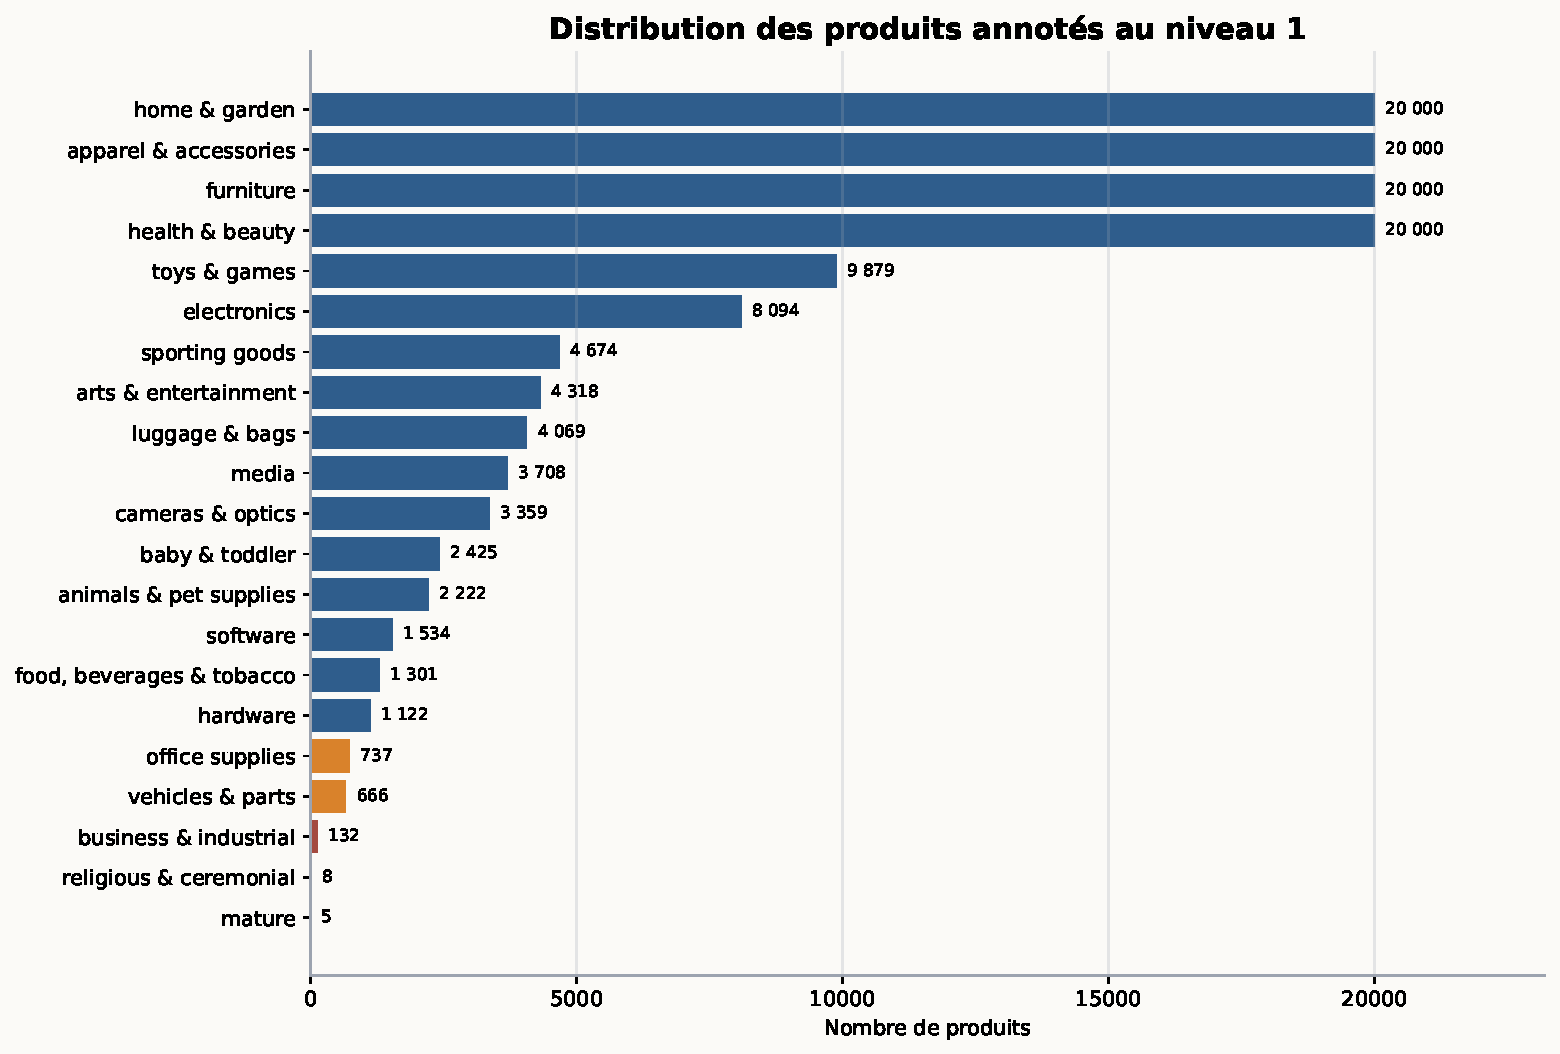
\includegraphics[width=\linewidth,height=0.74\textheight,keepaspectratio]{dataset_l1_distribution.pdf}
\end{column}

\begin{column}{0.34\textwidth}
\begin{block}{À retenir}
\begin{itemize}
    \item Fort déséquilibre entre classes.
    \item Plusieurs grandes catégories à 20\,000 produits.
    \item Catégories rares très peu représentées.
\end{itemize}
\end{block}

\begin{takeawaybox}
\centering
Une bonne micro-accuracy peut cacher de faibles performances sur les classes rares.
\end{takeawaybox}
\end{column}
\end{columns}
\end{frame}
% -----------------------------------------------------
\begin{frame}{Structure du fichier final}
\small
\begin{table}
\centering
\renewcommand{\arraystretch}{1.25}
\begin{tabular}{lll}
\toprule
\textbf{Colonne} & \textbf{Type} & \textbf{Rôle} \\
\midrule
\texttt{hashed\_external\_id} & Identifiant haché & Suivi et jointures \\
\texttt{text} & Texte consolidé & Entrée principale des embeddings \\
\texttt{sale\_price} & Numérique & Signal auxiliaire conservé \\
\texttt{level\_1\_name} & Label catégoriel & Supervision L1 \\
\texttt{brand\_encoded} & Marque encodée & Extension future possible \\
\bottomrule
\end{tabular}
\end{table}

\vspace{0.3cm}

\begin{takeawaybox}
\centering
Le texte devient la variable centrale ; prix et marque sont conservés comme signaux auxiliaires.
\end{takeawaybox}
\end{frame}

% -----------------------------------------------------
\begin{frame}{Transition -- Pourquoi enrichir les catégories ?}
\small
\begin{columns}
\begin{column}{0.48\textwidth}
\begin{block}{Problème}
\begin{itemize}
    \item Certains labels sont courts.
    \item Certains labels sont ambigus.
    \item Un nom unique couvre mal le vocabulaire produit.
\end{itemize}
\end{block}
\end{column}

\begin{column}{0.48\textwidth}
\begin{block}{Solution}
\begin{itemize}
    \item Plusieurs prototypes par catégorie.
    \item Nom canonique + enfants + variantes lexicales.
    \item Comparaison par similarité cosinus.
\end{itemize}
\end{block}
\end{column}
\end{columns}

\vspace{0.35cm}

\begin{takeawaybox}
\centering
On passe d'une catégorie représentée par \textbf{un seul point} à une catégorie représentée par \textbf{une région sémantique}.
\end{takeawaybox}
\end{frame}

% -----------------------------------------------------
\begin{frame}{Formalisation des prototypes enrichis}
\small
\begin{block}{Représentation d'une catégorie}
\[
P_c=
\left\{
p^{name}_c,\;
p^{children}_c,\;
p^{lex}_{c,1},\ldots,p^{lex}_{c,r}
\right\}
\]
\end{block}

\begin{block}{Score produit--catégorie}
\[
S(x,c)
=
\max_{p\in P_c}
\cos\big(f(x),f(p)\big)
\]
\end{block}

\begin{columns}
\begin{column}{0.49\textwidth}
\begin{itemize}
    \item \(x\) : produit
    \item \(c\) : catégorie
    \item \(P_c\) : prototypes de la catégorie
\end{itemize}
\end{column}

\begin{column}{0.49\textwidth}
\begin{itemize}
    \item \(f(x)\) : embedding produit
    \item \(f(p)\) : embedding prototype
    \item max : prototype le plus proche
\end{itemize}
\end{column}
\end{columns}

\vspace{0.2cm}

\begin{takeawaybox}
\centering
Le maximum évite de diluer le signal : un seul prototype pertinent peut suffire.
\end{takeawaybox}
\end{frame}

% -----------------------------------------------------
\begin{frame}{Recouvrement du manifold sémantique}
\small
\centering
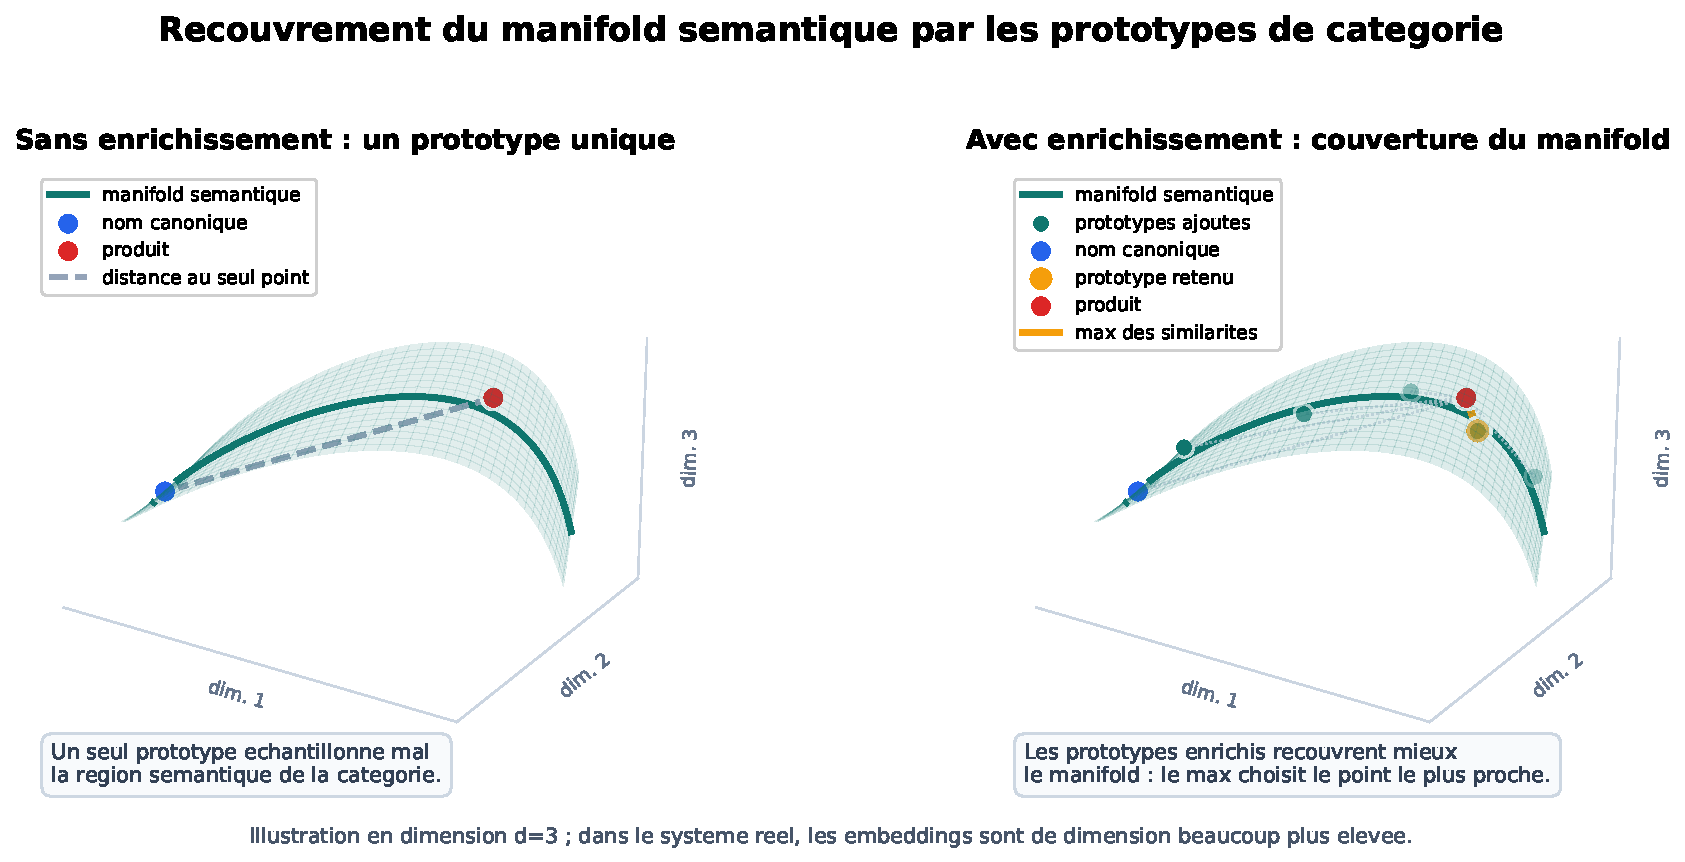
\includegraphics[width=0.93\linewidth,height=0.70\textheight,keepaspectratio]{category_prototype_manifold_coverage.pdf}

\vspace{0.15cm}

\begin{takeawaybox}
\centering
\textbf{Interprétation :} avec un seul prototype, la catégorie est mal couverte ; avec plusieurs prototypes, le produit peut trouver un voisin sémantique plus proche.
\end{takeawaybox}
\end{frame}
% -----------------------------------------------------
\begin{frame}{Catégories proches et prototypes multiples}
\small
\centering
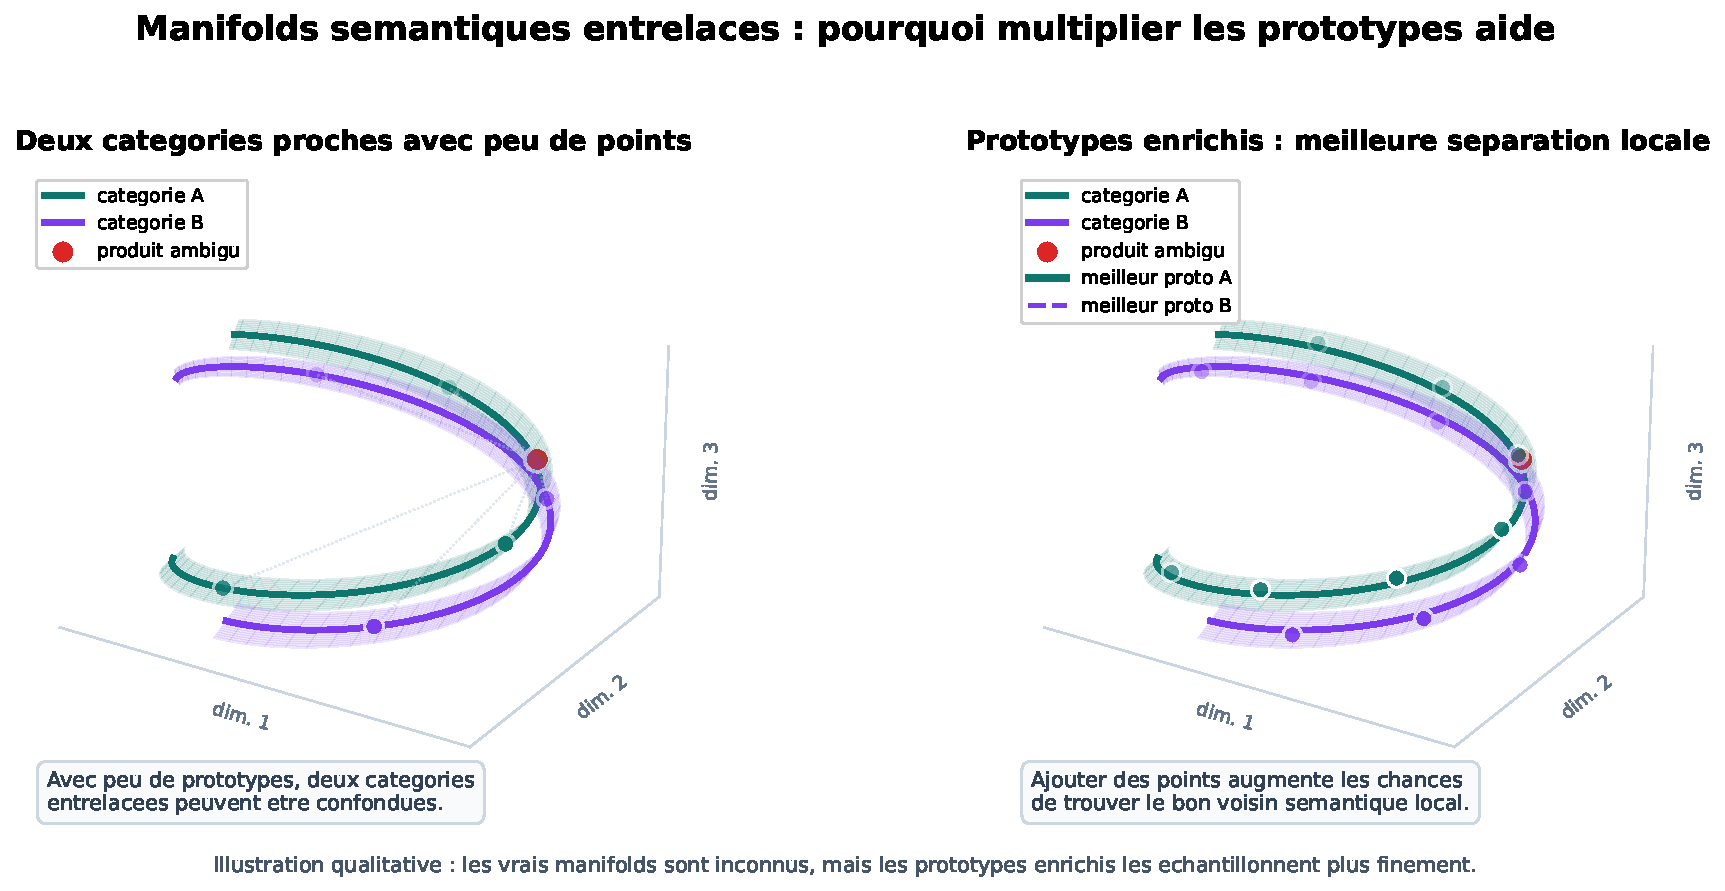
\includegraphics[width=0.93\linewidth,height=0.70\textheight,keepaspectratio]{category_interlaced_manifolds_enrichment.pdf}

\vspace{0.15cm}

\begin{takeawaybox}
\centering
\textbf{Interprétation :} lorsque deux catégories sont proches ou entrelacées, multiplier les prototypes augmente les chances de trouver le bon voisin sémantique local.
\end{takeawaybox}
\end{frame}
% -----------------------------------------------------
\begin{frame}{Synthèse de l'Axe 2}
\small
\begin{columns}
\begin{column}{0.49\textwidth}
\begin{block}{Ce que montre la Partie 3}
\begin{itemize}
    \item Base large : 128\,253 produits.
    \item Corpus anglophone : 99.89\%.
    \item Labels fiables seulement en L1.
    \item Taxonomie profonde : 5\,440 nœuds, 7 niveaux.
    \item Forte hétérogénéité des classes L1.
\end{itemize}
\end{block}
\end{column}

\begin{column}{0.49\textwidth}
\begin{block}{Ce que construit la Partie 4}
\begin{itemize}
    \item Représentation enrichie des catégories.
    \item Prototypes multiples par catégorie.
    \item Score par similarité cosinus maximale.
    \item Meilleure couverture du sens taxonomique.
    \item Base commune pour L1 et L2--L7.
\end{itemize}
\end{block}
\end{column}
\end{columns}

\vspace{0.30cm}

\begin{takeawaybox}
\centering
\textbf{Conclusion :} L'anlyse descritpive et l'enrichissement des catégories ont permis de transformer un catalogue brut en un espace textuel et sémantique exploitable pour la modélisation.
\end{takeawaybox}
\end{frame}

% =====================================================
% AXE 3 EMPTY
% =====================================================
\section{Axe 3 -- Catégorisation supervisée du Niveau 1}

\begin{frame}{Axe 3 -- Catégorisation supervisée du} 
\end{frame}

% =====================================================
% AXE 4 EMPTY
% =====================================================
\section{Axe 4 -- Zéro-shot L2--L7 et conclusion}

\begin{frame}{Axe 4 -- Du Niveau 1 supervisé aux niveaux profonds}
\small
\begin{columns}
\begin{column}{0.48\textwidth}
\begin{block}{Point de départ}
\begin{itemize}
    \item Le \textbf{Niveau 1} est appris par fine-tuning supervisé.
    \item Il sert de porte d'entrée dans le bon sous-arbre taxonomique.
    \item Il réduit fortement l'espace de recherche.
\end{itemize}
\end{block}
\end{column}

\begin{column}{0.48\textwidth}
\begin{block}{Changement de problème}
\begin{itemize}
    \item Les niveaux \textbf{L2 à L7} n'ont pas de ground truth fiable.
    \item On ne peut donc pas entraîner ni évaluer avec une accuracy classique.
    \item On passe à une logique de \textbf{recherche zéro-shot} dans la taxonomie.
\end{itemize}
\end{block}
\end{column}
\end{columns}

\vspace{0.3cm}

\begin{takeawaybox}
\centering
L'idée est donc : \textbf{prédire L1 proprement}, puis \textbf{affiner le chemin taxonomique sans supervision} à l'aide des embeddings et des catégories enrichies.
\end{takeawaybox}
\end{frame}

\begin{frame}{Méthodologie d'évaluation non supervisée}
\scriptsize
\renewcommand{\arraystretch}{1.18}
\begin{table}
\centering
\begin{tabular}{p{0.18\textwidth}p{0.26\textwidth}p{0.47\textwidth}}
\toprule
\textbf{Famille} & \textbf{Métriques} & \textbf{Ce que l'on mesure} \\
\midrule
Coût d'inférence & Temps total, ms / produit, débit, mémoire, millions d'opérations / produit & Viabilité opérationnelle du pipeline : latence, passage à l'échelle, coût vectoriel, charge mémoire. \\
Confiance interne & Marge top-1/top-2, profondeur moyenne, nombre de chemins, part du chemin majoritaire, entropie & Stabilité de la décision : un pipeline peut être profond mais peu fiable si plusieurs chemins restent presque ex-aequo. \\
Comparaison entre pipelines & Accord exact, accord niveau par niveau L2--L7, profondeur du premier désaccord, $V$ de Cramér & Cohérence relative entre méthodes sans vérité terrain. Un $V$ élevé avec un accord exact faible signifie une structure commune mais des chemins différents. \\
Audit NLP externe & Score bi-encodeur, score cross-encodeur, win rate, rang moyen & Préférence sémantique externe entre plusieurs chemins concurrents proposés pour un même produit. \\
\bottomrule
\end{tabular}
\end{table}

\vspace{0.2cm}

\begin{takeawaybox}
\centering
Sans accuracy L2--L7, on compare les pipelines par \textbf{coût}, \textbf{stabilité} et \textbf{cohérence relative}.
\end{takeawaybox}
\end{frame}

\begin{frame}{Pourquoi Qwen3 pour L2--L7 ?}
\small
\begin{table}
\centering
\scriptsize
\renewcommand{\arraystretch}{1.18}
\begin{tabular}{lrrrr}
\toprule
\textbf{Modèle} & \textbf{Dim.} & \textbf{Temps} & \textbf{Débit} & \textbf{Taille} \\
\midrule
Qwen3 & \textbf{1024} & 163.2 min & 17.0 txt/s & \textbf{650.6 MB} \\
Jasper & 2048 & \textbf{121.6 min} & \textbf{22.8 txt/s} & 1301.1 MB \\
\bottomrule
\end{tabular}
\end{table}

\vspace{0.25cm}

\begin{block}{}
\begin{itemize}
    \item Jasper encode plus vite, mais ses embeddings doublent le coût vectoriel et la mémoire.
    \item Qwen3 est plus favorable pour toutes les comparaisons produit--catégorie et produit--chemin.
    \item Le choix final est donc \textbf{Qwen3} pour la phase L2--L7.
\end{itemize}
\end{block}
\end{frame}

\begin{frame}{Pipeline 1 -- Décodage hiérarchique local}
\small
\begin{block}{Principe}
Après la prédiction du Niveau 1, on descend dans le sous-arbre correspondant. À chaque niveau, on compare le produit aux enfants du nœud courant.
\[
s(x,c)=\max_{p\in \mathcal{P}_c}\cos(g(x),g(p))
\]
\end{block}

\begin{columns}
\begin{column}{0.48\textwidth}
\begin{block}{Variantes}
\begin{itemize}
    \item \textbf{Greedy} : un seul chemin conservé.
    \item \textbf{Beam search} : plusieurs chemins candidats.
    \item \textbf{Beam + reranker} : reclassement final des meilleurs chemins.
\end{itemize}
\end{block}
\end{column}

\begin{column}{0.48\textwidth}
\begin{block}{Bilan}
\begin{itemize}
    \item Avantage : très naturel pour une taxonomie.
    \item Limite greedy : propagation d'erreur.
    \item Le beam corrige partiellement ce défaut, mais coûte plus cher.
\end{itemize}
\end{block}
\end{column}
\end{columns}
\end{frame}

\begin{frame}{Pipeline 2 -- Clustering hiérarchique}
\small
\begin{block}{Principe}
Dans une branche L1 donnée, on suppose que les produits des catégories enfants forment des groupes dans l'espace d'embeddings.
\[
\min_{\mu_1,\ldots,\mu_K}\sum_{i=1}^{n}\min_{k\in\{1,\ldots,K\}}\|z_i-\mu_k\|_2^2
\]
\end{block}

\begin{columns}
\begin{column}{0.48\textwidth}
\begin{block}{Étapes}
\begin{itemize}
    \item Lire dans la taxonomie le nombre d'enfants.
    \item Former ce nombre de clusters.
    \item Associer chaque centroïde à une catégorie enrichie.
\end{itemize}
\end{block}
\end{column}

\begin{column}{0.48\textwidth}
\begin{block}{Bilan}
\begin{itemize}
    \item Avantage : révèle une structure collective.
    \item Limite : une catégorie n'est pas toujours un cluster géométrique.
\end{itemize}
\end{block}
\end{column}
\end{columns}
\end{frame}

\begin{frame}{Pipeline 3 -- Recherche de chemins globaux}
\small
\begin{block}{Principe}
On encode les chemins complets L2--L7 une seule fois, puis on compare directement le produit à tous les chemins compatibles avec le Niveau 1 prédit.
\[
\hat{h}=\arg\max_{h\in\mathcal{H}(\hat{c}_1)}\cos(g(x),g(h))
\]
\end{block}

\begin{columns}
\begin{column}{0.48\textwidth}
\begin{block}{Intuition}
\begin{itemize}
    \item On évite les décisions locales irréversibles.
    \item Le chemin complet est évalué comme une hypothèse unique.
\end{itemize}
\end{block}
\end{column}

\begin{column}{0.48\textwidth}
\begin{block}{Bilan}
\begin{itemize}
    \item Avantage : plus diversifié, souvent plus profond.
    \item Limite : marges top-1/top-2 faibles entre chemins très proches.
    \item Très utile comme \textbf{méthode de désaccord}.
\end{itemize}
\end{block}
\end{column}
\end{columns}
\end{frame}

\begin{frame}{Résultats -- Coût et performance des pipelines}
\small
\begin{table}
\centering
\renewcommand{\arraystretch}{1.15}
\begin{tabular}{lrrrr}
\toprule
\textbf{Pipeline Qwen3} & \textbf{ms/prod.} & \textbf{M ops/prod.} & \textbf{Prof. moy.} \\
\midrule
Greedy & \textbf{1.14} & \textbf{0.39} & 3.08  \\
Beam & 2.71 & 0.62 & 3.22 \\
Beam + reranker & 16.17 & 0.62 + rerank & 3.21 \\
Clustering & 0.71 & 0.42 & 3.01  \\
Recherche globale & 1.67 & 0.51 & \textbf{3.37} \\
\bottomrule
\end{tabular}
\end{table}

\vspace{0.2cm}

\begin{takeawaybox}
\centering
\textbf{Greedy} est le meilleur compromis coût / latence ; \textbf{recherche globale} est la plus diversifiée ; \textbf{beam + reranker} apporte de la qualité brute mais change d'ordre de grandeur en coût.
\end{takeawaybox}
\end{frame}

\begin{frame}{Résultats -- Accord entre pipelines et V de Cramér}
\small
\begin{columns}
\begin{column}{0.54\textwidth}
\centering
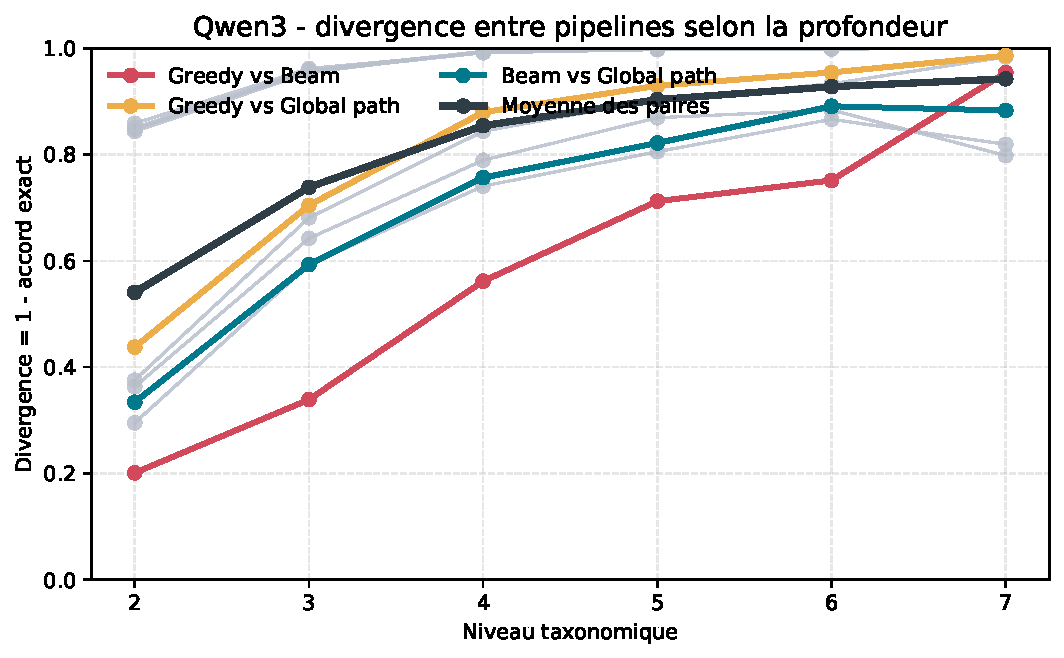
\includegraphics[width=\linewidth,height=0.70\textheight,keepaspectratio]{family3_divergence_by_depth_qwen.pdf}
\end{column}

\begin{column}{0.42\textwidth}
\begin{table}
\centering
\scriptsize
\renewcommand{\arraystretch}{1.15}
\begin{tabular}{lrr}
\toprule
\textbf{Métrique} & \textbf{Qwen3} & \textbf{Jasper} \\
\midrule
Même chemin & 1.3\% & 1.9\% \\
$V$ moyen & 0.426 & 0.446 \\
Même L2 & 15.0\% & 13.6\% \\
Même L3 & 13.1\% & 19.8\% \\
Dernier niv. commun & 2.49 & 2.46 \\
\bottomrule
\end{tabular}
\end{table}

\begin{block}{Bilan}
\begin{itemize}
    \item Faible accord exact.
    \item Mais association catégorielle non nulle.
    \item Les pipelines partagent souvent L2 puis divergent vite.
\end{itemize}
\end{block}
\end{column}
\end{columns}
\end{frame}

\begin{frame}{Résultats -- Audit NLP et intérêt du reranker}
\small
\begin{table}
\centering
\renewcommand{\arraystretch}{1.15}
\begin{tabular}{lrrr}
\toprule
\textbf{Scorer} & \textbf{Pipeline} & \textbf{Win Qwen} & \textbf{Rang Qwen} \\
\midrule
Bi-encodeur & Greedy & \textbf{29.5\%} & \textbf{2.50} \\
Bi-encodeur & Recherche globale & 20.1\% & 2.94 \\
Cross-encodeur & Greedy & 17.0\% & 2.92 \\
Cross-encodeur & Beam + reranker & \textbf{37.5\%} & \textbf{2.15} \\
\bottomrule
\end{tabular}
\end{table}

\vspace{0.25cm}

\begin{block}{Bilan}
\begin{itemize}
    \item Le \textbf{greedy} reste très compétitif en win rate.
    \item Le \textbf{beam + reranker} est le meilleur en qualité brute au cross-encodeur.
    \item Le reranker doit donc rester \textbf{sélectif}, pas systématique.
\end{itemize}
\end{block}
\end{frame}

\begin{frame}{Axe 4 -- Conclusion}
\small
\begin{columns}
\begin{column}{0.48\textwidth}
\begin{block}{Ce que l'on retient}
\begin{itemize}
    \item Qwen3 est l'encodeur retenu pour L2--L7.
    \item Le \textbf{greedy} est la baseline la plus crédible.
    \item Le \textbf{beam + global path + reranker} reste utile pour les cas ambigus.
\end{itemize}
\end{block}
\end{column}

\begin{column}{0.48\textwidth}
\begin{block}{Conclusion méthodologique}
\begin{itemize}
    \item Traiter tout le catalogue avec une méthode légère.
    \item Utiliser les désaccords entre pipelines comme signal d'incertitude.
    \item Réserver le reranking à une seconde passe ciblée.
\end{itemize}
\end{block}
\end{column}
\end{columns}

\vspace{0.35cm}

\begin{takeawaybox}
\centering
\textbf{Conclusion:} pour les niveaux 2 à 7, nous retenons un pipeline zéro-shot avec \textbf{Qwen3}, un \textbf{greedy} comme stratégie de base et un \textbf{reranking sélectif} uniquement pour les produits réellement ambigus.
\end{takeawaybox}
\end{frame}

\begin{frame}{Conclusion globale -- Ce que le projet apporte}
\small
\begin{columns}
\begin{column}{0.48\textwidth}
\begin{block}{Pipeline finale}
\begin{itemize}
    \item Catégories enrichies par prototypes textuels.
    \item \textbf{Level 1} supervisé avec \textbf{BGE-small} fine-tuné.
    \item \textbf{Levels 2--7} en zéro-shot avec \textbf{Qwen3}.
\end{itemize}
\end{block}
\end{column}

\begin{column}{0.48\textwidth}
\begin{block}{Idée centrale}
\begin{itemize}
    \item Garder une approche \textbf{compacte} et \textbf{peu coûteuse}.
    \item Utiliser la hiérarchie taxonomique comme contrainte.
    \item Réserver les méthodes coûteuses aux cas difficiles.
\end{itemize}
\end{block}
\end{column}
\end{columns}

\vspace{0.3cm}

\begin{takeawaybox}
\centering
Le projet propose une \textbf{méthodologie complète} : enrichissement, fine-tuning, pipelines zéro-shot, métriques non supervisées et benchmark de coût d'inférence.
\end{takeawaybox}
\end{frame}

\begin{frame}{Perspectives}
\small
\begin{columns}
\begin{column}{0.48\textwidth}
\begin{block}{Améliorations modèles}
\begin{itemize}
    \item Adapter davantage les embeddings au vocabulaire métier.
    \item Ajouter des signaux structurés comme le prix.
    \item Apprendre un reranker spécialisé sur la taxonomie Critéo.
\end{itemize}
\end{block}
\end{column}

\begin{column}{0.48\textwidth}
\begin{block}{Améliorations pipeline}
\begin{itemize}
    \item Construire un jeu annoté \textbf{L2--L7} pour une vraie évaluation supervisée.
    \item Utiliser des pseudo-labels à forte marge et de l'annotation active.
    \item Optimiser l'inférence à grande échelle : batchs, parallélisation, pré-calcul distribué.
\end{itemize}
\end{block}
\end{column}
\end{columns}

\vspace{0.25cm}

\begin{takeawaybox}
\centering
La suite naturelle du projet est de transformer une pipeline zéro-shot crédible en une pipeline \textbf{semi-supervisée}, progressivement validée par des labels profonds et optimisée pour le passage à l'échelle.
\end{takeawaybox}
\end{frame}

\begin{frame}{Travail en équipe et apport du projet}
\small
\begin{columns}
\begin{column}{0.48\textwidth}
\begin{block}{Travail en équipe}
\begin{itemize}
    \item Répartition des tâches entre data, modélisation, expérimentation et restitution.
    \item Aller-retour constants entre code, analyse et rapport.
    \item Construction progressive d'une pipeline cohérente malgré des contraintes fortes.
\end{itemize}
\end{block}
\end{column}

\begin{column}{0.48\textwidth}
\begin{block}{Ce que le projet nous a apporté}
\begin{itemize}
    \item Travailler sur un vrai problème industriel sous contrainte de coût.
    \item Concevoir une évaluation même sans ground truth complète.
    \item Relier recherche appliquée, engineering et communication des résultats.
\end{itemize}
\end{block}
\end{column}
\end{columns}

\vspace{0.3cm}

\begin{takeawaybox}
\centering
Ce projet nous a surtout appris à construire une solution \textbf{pragmatique et défendable}, en combinant rigueur méthodologique, expérimentation et travail collectif.
\end{takeawaybox}
\end{frame}

\end{document}
